\chapter{Introduction}\label{chap:introduction}

Sandia National Laboratories tests high-speed flight vehicles, such as sounding
rockets, reentry bodies, and guided missiles. \Cref{fig:taos-application} illustrates a
typical sounding-rocket test flight. These vehicles often travel at hypersonic
velocities and at high altitudes. The Trajectory Analysis and Optimization System
(TAOS) has been developed to calculate trajectories for this type of high-speed
vehicle; however, it can also be used for slower-speed vehicles, such as aircraft and
cruise missiles.

\begin{figure}[htbp]
  \centering
  \resizebox{0.86\linewidth}{!}{\begin{tikzpicture}[>=Latex,line cap=round,line join=round,font=\sffamily\scriptsize]
  % Reusable schematic rocket.
  \tikzset{
    rocket/.pic={
      \draw[line width=0.75pt] (0,-0.32) -- (0.13,0.20) -- (0,0.55)
        -- (-0.13,0.20) -- cycle;
      \draw[line width=0.75pt] (-0.13,0.18) -- (-0.25,-0.18) -- (-0.08,-0.08);
      \draw[line width=0.75pt] (0.13,0.18) -- (0.25,-0.18) -- (0.08,-0.08);
      \draw[line width=0.65pt] (-0.10,0.10) -- (0.10,0.10);
    }
  }

  % Main vehicle and payload trajectories.
  \draw[line width=1.15pt] (0.15,0.15)
    .. controls (0.70,2.55) and (1.45,4.15) .. (2.65,5.15);
  \draw[line width=1.15pt] (2.85,5.45)
    .. controls (4.50,6.55) and (7.00,5.20) .. (9.10,1.15);
  \draw[line width=1.05pt] (4.20,5.55)
    .. controls (6.05,4.35) and (7.05,2.60) .. (7.35,0.75);

  % Booster trajectory.
  \draw[line width=1.05pt] (2.35,3.55)
    .. controls (3.65,4.70) and (4.45,3.10) .. (4.55,1.10);

  % Vehicle icons.
  \pic[rotate=-18,scale=0.90] at (0.55,1.05) {rocket};
  \pic[rotate=-38,scale=0.72] at (2.40,4.65) {rocket};
  \pic[rotate=-40,scale=0.80] at (6.35,3.40) {rocket};
  \pic[rotate=-43,scale=0.62] at (7.25,4.25) {rocket};
  \pic[rotate=152,scale=0.68] at (4.05,3.05) {rocket};

  % Labels and event markers.
  \node[align=right] at (-0.05,0.65) {Rocket\\launch};
  \node[align=right] at (-0.25,1.65) {1st-stage\\burn};
  \node[align=right] at (1.10,3.35) {Staging};
  \node[align=right] at (1.75,4.85) {2nd-stage\\burn};
  \node[align=center] at (5.10,6.15) {Payload separation};
  \node[align=left] at (6.00,3.00) {2nd-stage\\trajectory};
  \node[align=left] at (7.65,4.20) {Payload\\trajectory};
  \node[align=left] at (4.35,2.75) {Booster\\trajectory};
  \node at (4.70,0.72) {Impact};
  \node at (7.40,0.35) {Impact};
  \node at (8.75,0.72) {Impact};
\end{tikzpicture}
}
  \caption{A TAOS application.}
  \label{fig:taos-application}
\end{figure}

TAOS predicts aircraft and missile trajectories from known vehicle characteristics.
Given a vehicle's mass, its initial conditions, and the forces acting on it, TAOS
computes its trajectory. A vehicle's trajectory is defined by its position, velocity,
and acceleration as a function of time. This information is used to determine a
vehicle's overall performance characteristics, such as its range, speed, time of
flight, and altitude. \Cref{fig:typical-trajectory-information} shows typical trajectory
information plotted as a function of time.

\begin{figure}[htbp]
  \centering
  \resizebox{0.96\linewidth}{!}{\begin{tikzpicture}
  \begin{axis}[
    name=altplot,
    width=6.25cm,height=4.1cm,
    xmin=0,xmax=240,ymin=0,ymax=100000,
    xtick={0,60,120,180,240},
    ytick={0,20000,40000,60000,80000,100000},
    grid=major,
    axis line style={line width=0.7pt},
    tick label style={font=\scriptsize},
    label style={font=\sffamily\scriptsize},
    xlabel={Flight time (sec)},
    ylabel={Altitude (ft)},
    ylabel style={align=center},
    scaled y ticks=false,
    yticklabel style={/pgf/number format/fixed,/pgf/number format/1000 sep={}},
  ]
    \addplot[line width=1.1pt,smooth] coordinates {
      (0,40000) (15,40500) (28,48000) (45,68000) (65,85000)
      (85,93000) (110,92000) (135,85000) (160,70000) (178,45000)
      (188,12000) (192,0)
    };
  \end{axis}

  \begin{axis}[
    at={($(altplot.east)+(1.55cm,0)$)},anchor=west,
    width=6.25cm,height=4.1cm,
    xmin=0,xmax=240,ymin=0,ymax=5000,
    xtick={0,60,120,180,240},
    ytick={0,1000,2000,3000,4000,5000},
    grid=major,
    axis line style={line width=0.7pt},
    tick label style={font=\scriptsize},
    label style={font=\sffamily\scriptsize},
    xlabel={Flight time (sec)},
    ylabel={Velocity (ft/sec)},
    ylabel style={align=center},
    scaled y ticks=false,
    yticklabel style={/pgf/number format/fixed,/pgf/number format/1000 sep={}},
  ]
    \addplot[line width=1.1pt,smooth] coordinates {
      (0,800) (18,2200) (34,4700) (47,4450) (75,4200) (110,4050)
      (145,3900) (175,3750) (188,3300) (194,2500)
    };
  \end{axis}
\end{tikzpicture}
}
  \caption{Typical trajectory information.}
  \label{fig:typical-trajectory-information}
\end{figure}

\section{Trajectory Simulation}\label{sec:trajectory-simulation}

The motion of an object relative to a fixed point in space is obtained from a set of
differential equations called the equations of motion. The equations of motion are
based on Newton's second law as applied to rigid bodies of constant mass:
\begin{equation}
  \begin{aligned}
    \sum \mathbf{F} &= m\mathbf{a}_{I}, &&\text{force equation},\\
    \sum \mathbf{M} &= \mathbf{I}\dot{\boldsymbol{\omega}}_{I}, &&\text{moment equation}.
  \end{aligned}
  \label{eq:force-equation}
\end{equation}
These equations represent a set of second-order differential equations that is
integrated with respect to time to compute an object's motion. The position and
velocity of the object's center of mass are obtained from the force equation, and the
object's angular orientation and rate are obtained from the moment equation. The two
inertial acceleration vectors each have three components, so there are six
second-order differential equations and the system is said to have six degrees of
freedom (6-DOF).

TAOS uses a simpler approach that assumes the vehicle has a control system,
automatic or human, capable of controlling the vehicle's angular orientation.
Therefore, angular orientation is assumed to be known and is supplied as an input
quantity. This assumption eliminates the moment equation and three degrees of
freedom. The problem reduces to
\begin{equation}
  \sum \mathbf{F}=m\mathbf{a}_{I},
  \label{eq:point-mass-force}
\end{equation}
which represents a set of three second-order differential equations for the motion of
a point mass. Thus, TAOS is often called a point-mass trajectory simulation or a
three-degree-of-freedom (3-DOF) simulation. The vehicle's position, velocity, and
acceleration depend on the forces acting on it and on its mass. Its angular orientation
is input, and it is assumed that a control system is capable of maintaining it. The
angular orientation is required to calculate the forces acting on the vehicle.

Although \Cref{eq:point-mass-force} is for a constant-mass rigid body, it can be used
for variable-mass bodies such as aircraft and rockets. Mass can change
instantaneously, for example when a weapon is dropped, and mass can change because
a propulsive system burns and exhausts fuel. An instantaneous mass change is handled
by dividing the trajectory into portions before and after the change. Mass changes
from a propulsive system produce propulsive and drag forces; these forces must be
included in the total force. An additional mass-flow equation is added to the set of
differential equations to provide user control over vehicle mass.

Over long time periods, control systems generally keep angular accelerations near
zero, a condition called trimmed flight. In a point-mass simulation the forces acting
on the vehicle must correspond to this trimmed condition. Trim forces used to
maintain the vehicle in various body orientations must be included as part of the total
force acting on the vehicle.

Point-mass, 3-DOF trajectory simulations can be calculated much faster than full
6-DOF simulations and require less information about the vehicle. This makes them
well suited to conceptual design, mission planning, and vehicle performance analysis.
They are excellent for predicting long-duration trajectory characteristics and overall
system performance. They cannot be used to study stability and control problems
involving the dynamic response of the vehicle and its control system, and they are
poorly suited to trajectories with large angular accelerations. Details of the
mathematical formulation used in TAOS are given in \Cref{chap:methods}.

\section{Development History}\label{sec:development-history}

The specific methods used in TAOS for flight-path prediction have a long history.
They began with development of the Point-Mass Simulation Tool (PMAST).\taosref{1} The
equations of motion, coordinate transformations, and preliminary code for PMAST
were derived by J. L. McDowell in 1984. This mathematical formulation was enhanced
and converted into usable software by the author during 1985. Because of its
capabilities and user interface, PMAST became widely used at Sandia for trajectory
prediction.

Parametric optimization methods vary a set of parameters to minimize an objective
function subject to constraints. These methods can vary the shape of a trajectory or
the timing of trajectory events to meet mission-planning and flight-path constraints.
Parametric optimization was tested in PMAST, but it was unreliable because of
singularities in the equations of motion and vehicle-attitude definitions. These
problems motivated development of a new version of the code.

During 1987 and 1988, D. E. Outka modified the equations of motion and mathematics
in PMAST, resulting in the Trajectory Simulation and Analysis Program (TSAP).\taosref{2} The
equations of motion in PMAST were derived in a wind coordinate system, which is
typical for aircraft trajectory simulations. Outka derived the TSAP equations of
motion in an earth-centered, earth-fixed coordinate system to avoid numerical
singularities. This method is commonly used for missile trajectories. Outka also used
unit vectors for coordinate transformations rather than transformation matrices and
improved the reliability and efficiency of the optimization procedure. The TSAP user
interface remained nearly identical to PMAST, and TSAP quickly became Sandia's
standard point-mass trajectory simulation software.

From 1988 to 1993, capabilities were added to TSAP as required to support flight-test
projects at Sandia. Problems involving multiple vehicles remained awkward, and TSAP
was not easy to adapt because of its program structure. In 1993 a decision was made
to develop a new multivehicle point-mass trajectory code.

The result was TAOS. Its mathematical formulation is nearly identical to TSAP, but
the primary change is extension to multiple vehicles. TAOS was written in the C
programming language rather than Fortran. C data structures and dynamic memory
allocation make it easier to extend from a single vehicle to multiple vehicles. The
user-interface style is similar to TSAP, but numerous changes support multivehicle
analysis, increase flexibility, and improve usability.

Numerical methods were also improved. Depending on the problem, single trajectories
without optimization require from approximately the same processing time to about
20 percent less time than TSAP. Long trajectories with optimization can run 50 to 60
percent faster. TAOS was designed for UNIX systems but was written in standard ANSI
C and could run on any computer system with a 32-bit C compiler. The source reports
that it was tested on an IBM personal computer running Windows NT with the Borland
C/C++ compiler. It required a 32-bit operating system and compiler, such as Windows
NT or VAX/VMS.

\section{Program Capabilities}\label{sec:program-capabilities}

TAOS is a general-purpose program capable of simulating many kinds of trajectories.
It divides a trajectory into pieces, called \emph{trajectory segments}, such that each
piece is relatively simple to describe.

\begin{figure}[htbp]
  \centering
  \resizebox{0.96\linewidth}{!}{\begin{tikzpicture}[>=Latex,line cap=round,line join=round,font=\sffamily\scriptsize]
  \coordinate (s0) at (0,0);
  \coordinate (s1) at (1.25,1.50);
  \coordinate (s2) at (2.10,2.55);
  \coordinate (s3) at (5.35,2.55);
  \coordinate (s4) at (6.40,2.55);
  \coordinate (s5) at (5.80,1.70);
  \coordinate (s6) at (6.80,1.50);
  \coordinate (s7) at (8.85,0.00);

  \draw[line width=1.15pt] (s0)
    .. controls (0.25,0.65) and (0.75,1.10) .. (s1)
    .. controls (1.45,2.10) and (1.75,2.45) .. (s2)
    -- (s3)
    .. controls (6.55,2.55) and (6.95,2.95) .. (s4)
    .. controls (6.55,2.10) and (6.10,1.75) .. (s5)
    .. controls (6.25,1.30) and (6.55,1.35) .. (s6)
    .. controls (7.55,1.20) and (8.25,0.60) .. (s7);

  \foreach \p in {s1,s2,s3,s4,s5,s6}{\fill (\p) circle (2.2pt);}
  \draw[->,line width=0.9pt] (-0.55,-0.35)--(0.05,0.15);
  \draw[->,line width=0.9pt] (9.35,-0.35)--(8.85,0.05);

  \node[align=left,below left] at (-0.45,-0.15) {Beginning of\\trajectory};
  \node[align=left,left] at (0.85,1.12) {Segment 1\\Constant flight-\\path-angle climb};
  \node[align=left,above] at (1.65,2.75) {Segment 2\\Constant-angle-of-\\attack pushover};
  \node[align=center,above] at (3.75,2.60) {Segment 3\\Level flight};
  \node[align=left,above] at (6.65,2.80) {Segment 4\\Level turn};
  \node[align=left,below] at (5.05,1.45) {Segment 5\\Level turn in the\\other direction};
  \node[align=left,right] at (6.95,1.85) {Segment 6\\Constant-$g$\\pushover};
  \node[align=left,right] at (8.05,0.65) {Segment 7\\Ballistic descent};
  \node[align=right,below right] at (9.40,-0.10) {End of\\trajectory};
\end{tikzpicture}
}
  \caption{Segmented trajectories.}
  \label{fig:segmented-trajectories}
\end{figure}

\Cref{fig:segmented-trajectories} shows a trajectory divided into seven segments.
Within each segment, the vehicle configuration and guidance rules remain unchanged.
When either changes, a new segment is defined. The segment trajectories are combined
to form the complete trajectory.

Guidance rules, for example ``fly level'' or ``fly at a constant angle of attack,''
determine the vehicle's angular orientation. Some rules directly specify orientation,
while others specify it indirectly. Because guidance rules change instantaneously
between segments, trajectories can have discontinuities in angular orientation. The
method assumes that these discontinuities are small and that the control system can
change rapidly from one orientation to another.

Multiple trajectories represent more than one vehicle or object. They can be used to
track spent boosters or deployed objects and to compute intercept trajectories.
\Cref{fig:multiple-trajectory-example} shows two trajectories that intercept.

\begin{figure}[htbp]
  \centering
  \resizebox{0.60\linewidth}{!}{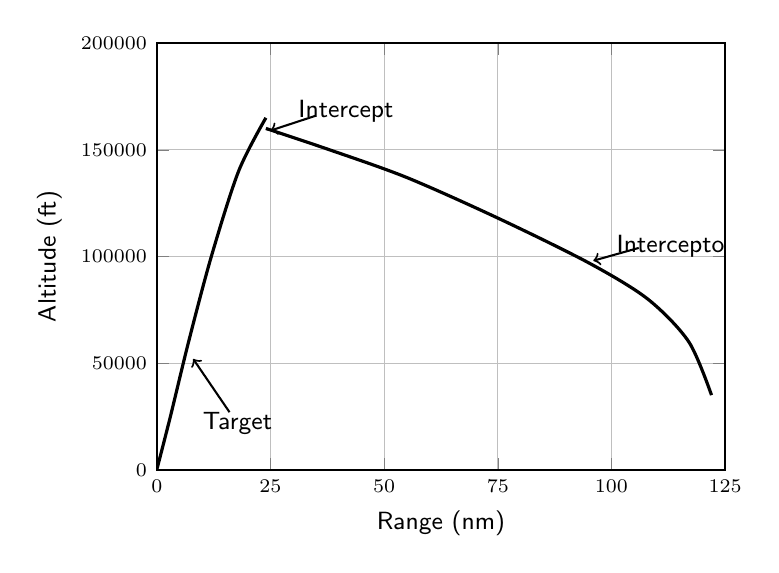
\begin{tikzpicture}
  \begin{axis}[
    width=8.8cm,height=7.0cm,
    xmin=0,xmax=125,ymin=0,ymax=200000,
    xtick={0,25,50,75,100,125},
    ytick={0,50000,100000,150000,200000},
    grid=major,
    axis line style={line width=0.8pt},
    tick label style={font=\scriptsize},
    label style={font=\sffamily\small},
    xlabel={Range (nm)},
    ylabel={Altitude (ft)},
    scaled y ticks=false,
    yticklabel style={/pgf/number format/fixed,/pgf/number format/1000 sep={}},
  ]
    \addplot[line width=1.15pt,smooth] coordinates {
      (0,0) (3,25000) (7,60000) (12,100000) (18,140000) (24,165000)
    };
    \addplot[line width=1.15pt,smooth] coordinates {
      (24,160000) (38,150000) (55,137000) (75,118000) (95,97000)
      (108,80000) (117,60000) (122,35000)
    };
    \node[font=\sffamily\small,anchor=west] at (axis cs:29,168000) {Intercept};
    \draw[->,line width=0.75pt] (axis cs:35,166000)--(axis cs:25,159000);
    \node[font=\sffamily\small,anchor=west] at (axis cs:99,105000) {Interceptor};
    \draw[->,line width=0.75pt] (axis cs:106,104000)--(axis cs:96,98000);
    \node[font=\sffamily\small,anchor=west] at (axis cs:8,22000) {Target};
    \draw[->,line width=0.75pt] (axis cs:16,27000)--(axis cs:8,52000);
  \end{axis}
\end{tikzpicture}
}
  \caption{A multiple-trajectory example.}
  \label{fig:multiple-trajectory-example}
\end{figure}

During conceptual-design studies, sets of trajectories are often computed while one
or more input parameters are systematically varied. TAOS provides a survey
capability for these tradeoff studies.

\subsection*{Parameter Optimization}

Mission planning and conceptual-design studies often require trajectories satisfying
many constraints. Parameter optimization varies selected input values to minimize an
objective function and satisfy those constraints. Optimization is the most powerful
feature in TAOS and gives the software great flexibility.

TAOS uses a parameter-optimization method called VF02, originally developed by
Powell.\taosref{3} This recursive quadratic programming method solves a general nonlinear
programming problem in which a set of parameters is varied to minimize an objective
function subject to equality and inequality constraints. Typical parameters include
initial conditions, guidance rules, and segment final conditions. Typical objective
functions include time, range, and altitude.

Simple constraints specify a value or limit for a trajectory variable, such as final
altitude, velocity, range, or flight-path angle. More complex constraints relate values
between trajectories. For example, an altitude in one trajectory can be constrained
to equal an altitude in another trajectory. Constraints can also apply to an entire
trajectory, such as maximum altitude or minimum dynamic pressure.

\section{Table and Problem Input Files}\label{sec:input-files}

The 1995 version of TAOS is a noninteractive program. All input data resides in one
or more files created before running TAOS, and output files are created during
execution. All input and output files are text files that can be created, inspected, and
modified with a text editor.

TAOS uses two types of input files: table files containing data such as thrust, mass
flow, and aerodynamic coefficients, and problem files containing trajectory-definition
data. Table filenames use the extension \texttt{.tbl}, and problem filenames use the
extension \texttt{.prb}. TAOS keys on these file types when processing input. Any
number of table and problem files can be supplied, although a typical run uses one or
two table files and one problem file.

\begin{center}
\begin{tabular}{lll}
\toprule
File type & Extension & Typical contents \\
\midrule
Table file & \texttt{.tbl} & Aerodynamics, propulsion, tabulated functions \\
Problem file & \texttt{.prb} & Initial/final conditions, trajectory description, print control \\
\bottomrule
\end{tabular}
\end{center}

Table files define forces acting on the vehicle and other quantities that are complex
functions of vehicle state. They usually remain constant for a given vehicle, so the
same table files are reused for many trajectories. Details are given in
\Cref{chap:table-files}. Problem files describe how trajectories are computed,
including initial conditions, segment definitions, and output descriptions. They are
generally smaller and change frequently. Their format is given in
\Cref{chap:problem-files}. A problem file is required; table files are optional because
constant aerodynamic and propulsive forces can be defined within a problem file.

\section{Program Execution}\label{sec:program-execution}

TAOS is executed from a UNIX shell or from DOS. On UNIX systems the command is
entered from a terminal or terminal window; on PC systems it is entered from a DOS
window. The command has the form
\begin{lstlisting}[language={},backgroundcolor=\color{white},frame=single]
taos file1.tbl file2.tbl ... filex.prb
\end{lstlisting}
The program name is followed by a list of table and problem filenames separated by
spaces. A full path may be required for the executable, for example:
\begin{lstlisting}[language={},backgroundcolor=\color{white},frame=single]
/usr/public/taos file1.tbl file2.tbl ... filex.prb
\end{lstlisting}
TAOS reads all table files first and then executes problem files in the order given.

On Silicon Graphics workstations used in Sandia's Aerospace Systems Development
Center, an icon was provided for TAOS. Input files could be selected, dragged to the
TAOS icon, and dropped to submit a batch job. Double-clicking the icon opened a
window containing the system batch-job list; the window was updated every five
seconds and could be left open to monitor job status continuously.

\begin{figure}[htbp]
  \centering
  \resizebox{0.72\linewidth}{!}{\begin{tikzpicture}[x=1cm,y=1cm,>=Latex,line cap=round,line join=round,font=\sffamily\small]
  \useasboundingbox (0,0) rectangle (10.2,3.85);
  \tikzset{
    fileicon/.pic={
      % Slightly three-dimensional document icon, closer to the workstation icon
      % printed in the source manual.
      \draw[line width=0.55pt] (0.10,0.07) -- (0.72,0.18) -- (0.72,0.96) -- (0.10,0.84) -- cycle;
      \draw[line width=0.85pt,fill=white] (0,0.14) -- (0.57,0.24) -- (0.57,1.02) -- (0,0.92) -- cycle;
      \draw[line width=0.65pt] (0.11,0.76)--(0.45,0.82);
      \draw[line width=0.65pt] (0.11,0.62)--(0.45,0.68);
      \draw[line width=0.65pt] (0.11,0.48)--(0.40,0.53);
      \draw[line width=0.65pt] (0.12,0.29) rectangle (0.43,0.43);
    },
    taosicon/.pic={
      % Stylized winged-flight icon and pedestal, preserving the visual role of
      % the historical Silicon Graphics TAOS desktop icon without embedding a raster.
      \draw[line width=0.85pt] (0.08,0.18)--(0.48,0.00)--(1.12,0.20)--(0.72,0.38)--cycle;
      \draw[line width=0.75pt] (0.42,0.31)--(0.63,0.50)--(0.78,0.33);
      \draw[line width=0.9pt] (0.58,0.36)
        .. controls (0.44,0.68) and (0.57,1.02) .. (0.94,1.24)
        .. controls (0.80,0.93) and (0.82,0.66) .. (0.99,0.43);
      \draw[line width=0.8pt] (0.72,0.88)--(0.20,1.05)--(0.55,0.78);
      \draw[line width=0.8pt] (0.79,0.83)--(1.32,1.02)--(0.96,0.73);
      \draw[line width=0.65pt] (0.84,1.13)--(1.07,1.34);
      \draw[line width=0.65pt] (0.88,1.10)--(1.20,1.18);
    }
  }

  \pic[scale=1.28] at (3.05,2.34) {fileicon};
  \node[anchor=north] at (3.41,2.36) {test.tbl};
  \pic[scale=1.28] at (3.05,0.28) {fileicon};
  \node[anchor=north] at (3.41,0.30) {test.prb};

  \pic[scale=1.32] at (6.45,1.10) {taosicon};
  \node[anchor=north] at (7.20,1.02) {taos};

  \node[align=left,anchor=west] (files) at (0.10,1.50) {Table and\\Problem File\\Icons};
  \draw[->,line width=0.95pt] (files.east) -- (2.86,2.82);
  \draw[->,line width=0.95pt] (files.east) -- (2.86,0.77);

  \node[align=left,anchor=west] (icon) at (8.62,2.54) {TAOS\\Icon};
  \draw[->,line width=0.95pt] (icon.west) -- (7.63,2.08);
\end{tikzpicture}
}
  \caption{TAOS Icon on Silicon Graphics Workstations.}
  \label{fig:taos-icon}
\end{figure}

As TAOS calculates each trajectory, it saves output data in memory. The original
manual notes typical requirements of 4 to 16 MB, depending on trajectory length,
integration step size, and print interval. This could constrain smaller PC systems of
the period.

\section{Output Files}\label{sec:output-files}

TAOS automatically creates printout files. A printout file has the same base name as
the input problem file and the extension \texttt{.out}. A separate printout file is
created for each problem file. It always contains a listing of the problem file and
error messages; the remaining content is controlled by the problem file, including
the variables printed and the print interval.

\begin{figure}[htbp]
  \centering
  \begin{minipage}{0.95\linewidth}
\centering
{\ttfamily\fontsize{6.15}{7.05}\selectfont
\begin{tabular*}{0.96\linewidth}{@{}l@{\extracolsep{\fill}}c@{}}
Sandia National & Trajectory Analysis \& Optimization Software\\[-1pt]
Laboratories & (TAOS -- Version 96.0)
\end{tabular*}

\vspace{1pt}
\noindent\makebox[0.96\linewidth][l]{\leaders\hbox{-}\hfill\kern0pt}
\vspace{3pt}

\textbf{Example of a ballistic reentry-body trajectory}\\[2pt]
Problem (ballistic) / 1976 US Standard Atmosphere / Non-rotating WGS-84 Earth\\[3pt]
Trajectory for vehicle: rv\\[3pt]

\setlength{\tabcolsep}{4.35pt}
\begin{tabular}{rrrrrrr}
Time & Alt & Range & Long & Mach & Vel & Gamgd\\
0.000 & 300000.0 & 0.000 & 20.00000 & 19.9642 & 18000.00 & -25.000\\
0.500 & 296194.1 & 1.324 & 20.02202 & 19.9715 & 18006.57 & -25.023\\
1.000 & 292383.5 & 2.648 & 20.04405 & 19.9788 & 18013.14 & -25.046\\
1.500 & 288568.3 & 3.973 & 20.06609 & 19.9861 & 18019.71 & -25.069\\
2.000 & 284748.3 & 5.298 & 20.08814 & 19.9933 & 18026.27 & -25.092\\
2.500 & 280923.7 & 6.623 & 20.11019 & 20.0006 & 18032.82 & -25.115\\
3.000 & 277094.4 & 7.949 & 20.13225 & 19.9008 & 18039.37 & -25.138\\
3.500 & 273260.5 & 9.276 & 20.15432 & 19.7897 & 18045.91 & -25.161\\
4.000 & 269421.8 & 10.603 & 20.17640 & 19.6805 & 18052.43 & -25.184\\
4.500 & 265578.5 & 11.930 & 20.19848 & 19.5731 & 18058.93 & -25.207\\
5.000 & 261730.6 & 13.258 & 20.22057 & 19.4673 & 18065.42 & -25.230\\
5.500 & 257878.0 & 14.587 & 20.24267 & 19.3632 & 18071.89 & -25.253\\
6.000 & 254020.7 & 15.915 & 20.26478 & 19.2606 & 18078.32 & -25.276\\
6.500 & 250158.9 & 17.245 & 20.28690 & 19.1597 & 18084.73 & -25.299\\
\end{tabular}
}
\end{minipage}

  \caption{Example Printout.}
  \label{fig:example-printout}
\end{figure}

TAOS also writes status information and error messages to standard output. On UNIX
systems this information can be redirected to a file. When the Silicon Graphics icon
is used, it is written to the batch-job output file.

Two additional output formats can be created: files containing trajectory values
formatted for the Engineering Graphics System (EGS),\taosref{4} and files containing trajectory
values arranged in columns. EGS was used to produce the trajectory plots in the
original report. Column-oriented files can be plotted with other software and are
also useful for exchanging trajectory information.

\section{Future Plans}\label{sec:future-plans}

The original manual anticipated interactive creation and editing of table and problem
files, including interactive plotting of tabulated data to help users avoid input errors.
It also anticipated interactive plotting of trajectory output during execution so that
long optimization runs could be observed and stopped if they were not working
correctly. Finally, as with PMAST and TSAP, new output variables and guidance rules
were expected to be added as required to support Sandia projects.
